\documentclass[12pt, a4paper]{article}
\PassOptionsToPackage{sharp}{prettytex/boxes}
\usepackage{prettytex/base}

\setlength{\topmargin}{0.0in}
\setlength{\oddsidemargin}{0.33in}
\setlength{\textheight}{9.0in}
\setlength{\textwidth}{6.0in}
\renewcommand{\baselinestretch}{1.25}

\usepackage{prettytex/math}
\usepackage{prettytex/math-theorems}
\usepackage{prettytex/mathematicians}
\usepackage{prettytex/gfx}
\usepackage{prettytex/code}
\usepackage{prettytex/thesis}
\usepackage{cleveref}
\usepackage{lipsum}

\setlength{\headheight}{19.53pt}
\setlength{\headsep}{1.8em}
\setlength{\belowcaptionskip}{-12pt}
\addbibresource{sources.bib}

\newcommand{\topictitle}{Solving PDEs using Spectral Methods in the Chebyshev basis \\ \large by example of the Heat Equation}
\newcommand{\candidatenumber}{12345}
\newcommand{\course}{Approximation of Functions}

\title{\topictitle}
\author{Candidate \candidatenumber}
\date{\today}

% Outline:
% Setting: define heat equation PDE problem (with BCs), explain series in x direction
% ✅ Introduce Chebyshev polynomials (relation of x, z and theta)
% ✅ Prove recurrence relation
% ✅ Prove orthogonality
% ✅ - Using transformation to theta
% ✅ - cite Cauchy integral for Laurent series
% ✅ Define Lipschitz
% Define Function Space in Cheb Basis
% ✅ Introduce Cheb series
% Algorithm one: interpolantThrough()
% - Method one: Rectangular integral approx. rule
% - Method two: DCT
% - Method three: Barycentric formula
% Algorithm two: evaluateOn()
% Numerics: Define Forward Euler
% Algorithm three: differentiation of a Cheb series
% - Method one: via DCT (todo...)
% - Method two: via recursion formula
% - Method three: via finite differences and repeated interpolantThrough()
% Final application: interpolantThrough(), u_1 = alpha * dt * diff(diff(u_0)), evaluateOn()
% Results

\begin{document}
  \pagestyle{plain}
  \begin{center}
    \vspace*{-2.5cm}
    \Large \topictitle \\
    \vspace{.3cm}

    \normalsize Special Topic on \textcolor{themecolor3}{\textsc{\course}}\\
    \normalsize Candidate Number: \textcolor{themecolor3}{\candidatenumber}
    \vspace{.3cm}
  \end{center}

  \begin{abstract}
    This work shall attempt to numerically solve the heat equation $u_t = \alpha u_{xx}$ with Dirichlet boundary conditions over the domain $[-1, 1] \times [0, T]$ by representing the spatial component as a \textit{Chebfun} (Chebyshev series) and moving on in time by the Forward Euler method.

    The implementation, centered around what we will refer to as \textbf{\textcolor{themecolor3}{TschebFun}}, including three major algorithms \texttt{\textcolor{themecolor3}{TschebFun}::\textcolor{themecolor2}{interpolantThrough}()}, \texttt{\textcolor{themecolor3}{TschebFun}::\textcolor{themecolor2}{evaluateOn}()} and \texttt{\textcolor{themecolor3}{TschebFun}::\textcolor{themecolor2}{derivative}()}, is done manually in C++, extended to work as a Python module and for demonstration, even features a high-level graphical interface to play with.
    Finally, we will compare the numerical results with the output of \textit{Chebfun}'s high-level \texttt{pde15s()}.
  \end{abstract}

  \textbf{Goal:}
  Numerically obtain the solution $u(x, T)$ of
  $$\begin{cases}
      \frac{\partial u}{\partial t} = \alpha \frac{\partial^2 u}{\partial x^2} \quad & u: [-1, 1] \times [0, T] \mapsto \R,\, T \in \R^+,\; \alpha \in \R\backslash\{0\} \\
      u(x_j, 0) = u_0(x_j) \quad                                                     & \forall x_j \in X_N,\; N \in \N,\, N > 1, \; u_0: [-1, 1] \mapsto \R              \\
      u(b, t) = u_0(b)                                                               & \forall b \in \{-1, 1\},\; \forall t \in [0, T] \,.
    \end{cases}$$

  \begin{figure}[H]
    \centering
    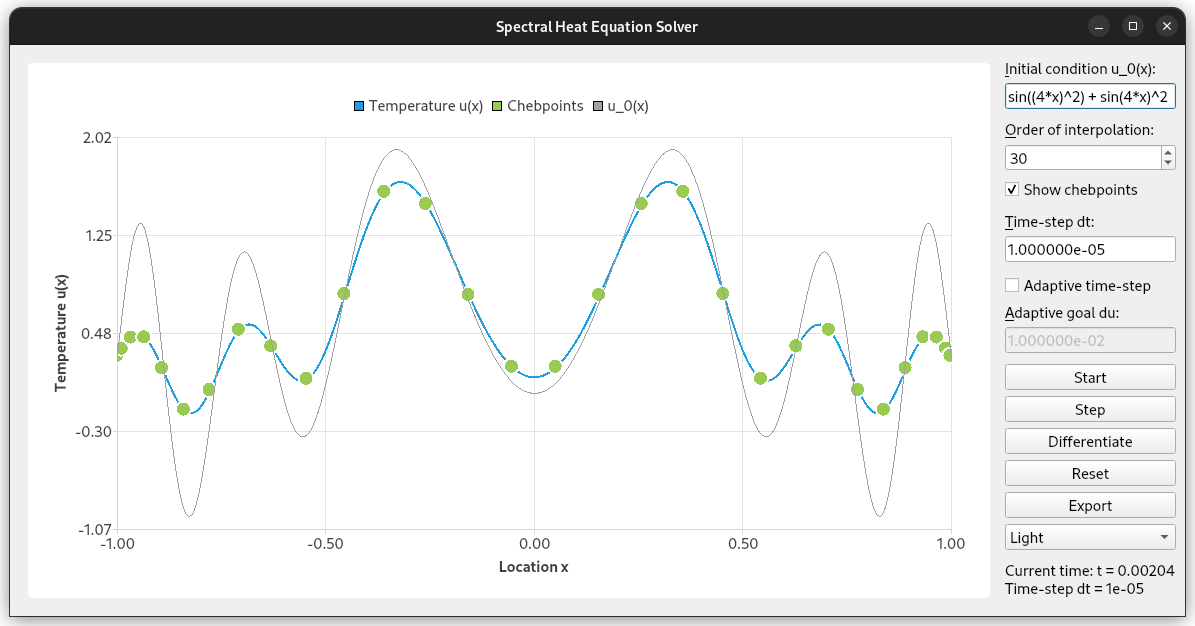
\includegraphics[width=0.8\linewidth]{figures/screenshot.png}
    \caption{Screenshot of the graphical user interface}
  \end{figure}

  \pagebreak
  \pagestyle{normal}

  \section{Motivation}
  Partial differential equations are notoriously hard to solve. One more possible approach to make way in this important class of problems is by the technique of spectral methods, incidentally closely related to finite element methods.
  The key idea is to perform the problem solution by representation of the occurring functions in a certain basis.
  For non-periodic problem settings, \textsc{Chebyshev} series are a fantastic choice.

  \section{Chebyshev and why we like his polynomials}
  Let $\N$ denote the nonnegative integers, so $0 \in \N$.

  \begin{definition}{Chebyshev polynomial}{chebpoly}
    Chebyshev\footnote{named after Pafnuty Lvovich \textsc{Chebyshev}, alternatively transliterated as Tchebycheff, Tchebyshev (French) or \textsc{Tschebyschow} (German)} polynomials $T_k: \R \mapsto \R$ are functions satisfying
    \begin{align*}
      T_k(x) = T_k(\cos \theta) := \cos(k \theta) = \frac{1}{2} (z^k + z^{-k}) \\
      z := \e^{i \theta},\quad x := \Re(z) = \cos(\theta) = \frac{1}{2}(z + z^{-1})
    \end{align*}
    for $k \in \N$. Then, $T_0(x) = 1$, $T_1(x) = x$, $T_2(x) = 2x^2-1$, and so on.
  \end{definition}

  These relations between $x$, $z$ and $\theta$ reveal fundamental connections between three famous basis sets (as we will confirm later): \textsc{Chebyshev}, \textsc{Laurent} and \textsc{Fourier}.

  \begin{theorem}{Chebyshev Recursion Formula}{chebrecursion}
    The Chebyshev polyomials satisfy the three-term recurrence relation $$T_{k+1}(x) = 2x T_k(x) - T_{k-1}(x) \,.$$
  \end{theorem}
  \begin{proof}{\autoref{thm:chebrecursion}}
    For $k > 1$,
    \begin{align*}
      2x T_k(x) - T_{k-1}(x) & = 2x \frac{1}{2} (z^k + z^{-k}) - \frac{1}{2} (z^{k-1} + z^{-(k-1)})                       \\
                             & = 2 \frac{1}{2}(z + z^{-1}) \frac{1}{2}(z^k + z^{-k}) - \frac{1}{2} (z^{k-1} + z^{-k+1})   \\
                             & = \frac{1}{2} (z^{k+1} + z^{k-1} + z^{-k+1} + z^{-k-1}) - \frac{1}{2} (z^{k-1} + z^{-k+1}) \\
                             & = \frac{1}{2} (z^{k+1} + z^{-(k+1)}) = T_{k+1}(x)
    \end{align*}
  \end{proof}

  The Chebyshev polynomials also satisfy an \emph{orthogonality relation},
  $$\langle T_m, T_n \rangle := \int_{-1}^1 T_m(x) T_n(x) \frac{1}{\sqrt{1-x^2}} \ddx = \int_{\pi}^{0} \cos(m \theta) \cos(n \theta) \frac{-\sin(\theta)}{\sqrt{1-\cos^2(\theta)}} \dd\theta \,,$$
  which becomes, with the fitting substitution $x = \cos(\theta)$ and $\ddx = -\sin(\theta) \dd\theta$,
  \begin{align*}
    \langle T_m, T_n \rangle & = \int_0^\pi T_m(\cos \theta) T_n(\cos \theta) \frac{\sin \theta}{\sin \theta}\dd\theta = \int_0^\pi \cos(m \theta) \cos(n \theta) \dd\theta                            \\
                             & = \frac{1}{2} \int_0^\pi \big(\underbrace{\cos((m+n) \theta)}_{=\cos(2m\theta) \text{ for } m=n} + \underbrace{\cos((m-n) \theta)}_{=1 \text{ for } m=n}\big) \dd\theta
  \end{align*}
  along with the knowledge that $\int_0^\pi \cos(k \theta) \dd\theta = k^{-1} \left[\sin(k\theta)\right]_0^\pi = 0$ for $k \in \Z \backslash \{0\}$,
  $$\langle T_m, T_n \rangle = \int_0^\pi T_m(\cos \theta) T_n(\cos \theta) \dd\theta = \begin{cases}
      0     & \text{ for } m \neq n     \\
      \pi/2 & \text{ for } m = n \neq 0 \\
      \pi   & \text{ for } m = n = 0
    \end{cases}$$
  which can be effectively utilised to define a function space $(\mathcal{T}, +, \cdot)$ in the \emph{orthogonal} basis of Chebyshev polynomials $\mathcal{T} := \{T_k\}_{k \in \N}$.
  Note that the operation $\langle \cdot, \cdot \rangle$ satisfies all axioms of an authentic inner product (linearity, etc.) over a function space due to the linearity of the integral.

  In the following proceedings, we will restrict our view on functions over the interval $[-1, 1] \subset \R$.
  Any (real) Lipschitz-continuous function $f \in \mathcal{C}_L$, where $\cC_L := \{g: [-1, 1] \mapsto \R \;|\; \exists L \text{ s.t. } \forall x_1, x_2 \in \R, \; |g(x_1) - g(x_2)| \le L \cdot |x_1-x_2|\}$ can be represented in the Chebyshev basis $\cT$, as Lipschitz continuity is a sufficient condition for absolute and uniform convergence of the corresponding series representation
  $$f(x) = \sum_{k=0}^\infty a_k T_k(x), \quad a_k \in \R,\quad k \in \N \,.$$

  Utilising orthogonality, for any $f \in \cC_L$, we find coefficients $a_l \in \R$ by 'right-multiplying' the equation $f = \sum_{k=0}^\infty a_k T_k$ with any one of the Chebyshev polynomials $T_l$.
  \begin{align*}
    \langle f, T_l \rangle & = \langle \sum_{k=0}^\infty a_k T_k, T_l \rangle = \int_0^\pi a_k T_k(\cos \theta) T_l(\cos \theta) \dd\theta \\
                           & = \sum_{k=0}^\infty a_k \langle T_k, T_l \rangle \quad \text{ \textcolor{gray}{by linearity}}                 \\
                           & = \begin{cases}
                                 a_0 \pi   & \text{ for } l = 0    \\
                                 a_l \pi/2 & \text{ for } l \neq 0
                               \end{cases}
  \end{align*}
  which can easily be rearranged to give explicit relations for $a_0$ and $a_k$
  \begin{align*}
    a_0 & = \frac{1}{\pi} \langle f, T_0 \rangle =  \frac{1}{\pi} \int_0^\pi f(\cos \theta) \dd\theta                                   \\
    a_k & = \frac{2}{\pi} \langle f, T_k \rangle = \frac{2}{\pi} \int_0^\pi f(\cos \theta) \cos(k \theta) \dd\theta, \quad k \neq 0 \,.
  \end{align*}
  Dealing with a numerical problem, we shall approximate the above two integrals by the rectangular integral rule.
  A different approach for the derivation of the explicit coefficient integrals can be found in \cite{atap} along with a complex analysis styled proof.

  \begin{theorem}{Rectangular integral rule}{integralapprox}
    $$\int_a^b f(x) \ddx = \lim_{N \rightarrow \infty} \frac{b-a}{N} \sum_{k=0}^N f(x_k), \quad x_k := a + \frac{b-a}{N} k$$
  \end{theorem}
  \cite[128]{bonthuis-cp}

  Most importantly, this quadrature-style integral approximation is only one way of numerically determining the coefficients $a_k$.
  Another is to recognise the structure of the above integral for $k \neq 0$ as a cosine transform of the function $(f \circ \cos)$.

  \begin{definition}{Cosine Transform}{costrans}
  \end{definition}

  \begin{definition}{Discrete Cosine Transform}{dct}
  \end{definition}

  Most significantly, this approach via the Discrete Cosine Transform can be sped up by means of the \emph{Fast Fourier Transform} \parencite{cooley-tukey-fft}.

  Numerically speaking, a significant improvement to these two approaches can be made by using the \emph{Barycentric interpolation formula in Chebyshev points} \parencite{atap}.
  Given more time, one should implement this feature in TschebFun as well.

  \begin{definition}{Chebyshev points}{chebpoints}
    From the equispaced points
    $$\Theta_N := \{\theta_j := jN/\pi \;|\; j = 0, ..., N\} \,,$$
    we can further define the Chebyshev points as the corresponding $\cos(\theta_j)$,
    $$X_N := \{x_j := \cos(\theta_j) \;|\; \theta_j \in \Theta_N\} \,.$$
  \end{definition}

  \begin{figure}[H]
    \centering
    \inputtikz{chebpoints}
    \caption{The Chebyshev points $\{x_j = \cos(\theta_j)\}$ are projections of the equispaced points $\{\theta_j\}$ on the unit circle onto the x-axis.}
  \end{figure}

  \inputminted{cpp}{../solver/TschebFun.h}

  One way of forcing the boundary conditions, at least the first that came to my mind when thinking of this issue, is to pin down the two highest-order coefficients in the series representation.

  \section{The heat equation and its solution}
  \section{Differentiation}
  \section{Results}
  \begin{figure}[H]
    \centering
    \inputtikz{numerical-comparison}
    \caption{Comparison of heatfun and chebfun}
  \end{figure}

  \section{Discussion}

  \printbibliography

  \appendix
  \section{Title of Appendix}
  Appendices are definitely not necessary and assessors are not obliged to read them so only use them for non-vital text, figures or calculations.
\end{document}
